% !TEX TS-program = latex
% !TEX spellcheck = it-IT
\documentclass[a4paper]{article}
\usepackage[utf8]{inputenc}
\usepackage[T1]{fontenc}
\usepackage[italian]{babel}
\usepackage{tikz} % LATEX
\usetikzlibrary {automata}


%%%%%%%%%%%%%%%%%%%%%%%%%%%%%%%%%%%%%%%%%%%%%%%%%%%%%%%%%%%%%%%%%%%%%%%%%%%%
%% Trim Size: 9.75in x 6.5in
%% Text Area: 8in (include Runningheads) x 5in
%% ws-ijgmmp.tex   :   2-9-08
%% Tex file to use with ws-ijgmmp.cls written in Latex2E.
%% The content, structure, format and layout of this style file is the
%% property of World Scientific Publishing Co. Pte. Ltd.
%% Copyright 1995, 2002 by World Scientific Publishing Co.
%% All rights are reserved.
%%%%%%%%%%%%%%%%%%%%%%%%%%%%%%%%%%%%%%%%%%%%%%%%%%%%%%%%%%%%%%%%%%%%%%%%%%%%
%%

%%%%%%%%%%%%%%%%%%%%%%%%%%%%%


\usepackage{pictexwd,dcpic}
\usepackage{csquotes}
\usepackage{nopageno}

\usepackage{amsmath, amssymb, amsthm}
\usepackage{pictex, dcpic}
\usepackage{color}
%\usepackage{graphicx}
%\numberwithin{equation}{section} % This line resets equation numbering when starting a new section.
%\renewcommand{\theequation}{Eq. \thesection.\arabic{equation}} % This line ads "Eq." in front of your equation numbering.




%
%    Macros.    Version 1.2.0.beta
%    The best use is to paste all of them into the papers
%     1/8/2005
%

%%%%%%%%%%%%%%%%%%%%%%%%%%%%%%
%%%%%%			Greek		 %%%%%%
%%%%%%%%%%%%%%%%%%%%%%%%%%%%%%

\def\al{\alpha}
\def\be{\beta}
\def\de{\delta}
\def\ga{\gamma}
\def\up{\upsilon}
\def\ep{\epsilon}
\def\io{\iota}
\def\te{\theta}
\def\la{\lambda}
\def\ze{\zeta}
\def\om{\omega}
\def\si{\sigma}
\def\vp{\varphi}
\def\vpi{\varpi}
\def\ka{\kappa}
\def\vs{\varsigma}
\def\vr{\varrho}

\def\De{\Delta}
\def\Ga{\Gamma}
\def\Te{\Theta}
\def\La{\Lambda}
\def\Om{\Omega}
\def\Si{\Sigma}
\def\Up{\Upsilon}

\def\boldDe{\bf\Delta}
\def\boldGa{\bf\Gamma}
\def\boldTe{\bf\Theta}
\def\boldLa{\bf\Lambda}
\def\boldOm{\bf\Omega}
\def\boldSi{\bf\Sigma}
\def\boldUp{\bf\Upsilon}
\def\boldXi{\bf\Xi}
\def\boldPi{\bf\Pi}
\def\boldPhi{\bf\Phi}
\def\boldPsi{\bf\Psi}

\def\boldal{\bf\al}
\def\boldbe{\bf\be}
\def\boldga{\bf\ga}
\def\boldde{\bf\de}
\def\boldep{\bf\ep}
\def\boldze{\bf\ze}
\def\boldeta{\bf\eta}
\def\boldte{\bf\te}
\def\boldio{\bf\io}
\def\boldka{\bf\ka}
\def\boldla{\bf\la}
\def\boldmu{\hbox{\greekbold\char "16}}
\def\boldnu{\hbox{\greekbold\char "17}}
\def\boldxi{\hbox{\greekbold\char "18}}
\def\boldpi{\hbox{\greekbold\char "19}}
\def\boldrho{\hbox{\greekbold\char "1A}}
\def\boldsi{\bf\si}
\def\boldtau{\hbox{\greekbold\char "1C}}
\def\boldup{\hbox{\greekbold\char "1D}}
\def\boldphi{\hbox{\greekbold\char "1E}}
\def\boldchi{\hbox{\greekbold\char "1F}}
\def\boldpsi{\hbox{\greekbold\char "20}}
\def\boldom{\hbox{\greekbold\char "21}}
\def\boldvep{\hbox{\greekbold\char "22}}
\def\boldvte{\hbox{\greekbold\char "23}}
\def\boldvpi{\hbox{\greekbold\char "24}}
\def\boldvrho{\hbox{\greekbold\char "25}}
\def\boldvsi{\hbox{\greekbold\char "26}}
\def\boldvphi{\hbox{\greekbold\char "27}}

%%%%%%%%%%%%%%%%%%%%%%%%%%%%%%
%%%%%%			Cal			 %%%%%%
%%%%%%%%%%%%%%%%%%%%%%%%%%%%%%
 \def\calA{{\hbox{\cal A}}}
 \def\calU{{\hbox{\cal U}}}
 \def\calB{{\hbox{\cal B}}}
 \def\calC{{\hbox{\cal C}}}
 \def\calI{{\hbox{\cal I}}}
 \def\calQ{{\hbox{\cal Q}}}
 \def\calP{{\hbox{\cal P}}}
 \def\calL{{\hbox{\cal L}}}
 \def\calE{{\hbox{\cal E}}}
 \def\calW{{\hbox{\cal W}}}
 \def\calV{{\hbox{\cal V}}}
 \def\calS{{\hbox{\cal S}}}
 \def\calF{{\hbox{\cal F}}}
 \def\calR{{\hbox{\cal R}}}
 \def\calO{{\hbox{\cal O}}}
 \def\calM{{\hbox{\cal M}}}

%%%%%%%%%%%%%%%%%%%%%%%%%%%%%%
%%%%%%			gothic		 %%%%%%
%%%%%%%%%%%%%%%%%%%%%%%%%%%%%%
 \def\su{{\mathfrak{su}}}
 \def\gl{{\mathfrak{gl}}}
 \def\gotg{{\mathfrak{g}}}
 \def\goth{{\mathfrak{h}}}
 \def\gotm{{\mathfrak{m}}}
 \def\gotk{{\mathfrak{k}}}
 \def\spin{{\mathfrak{spin}}}
 \def\slC{{\mathfrak{sl}}}
 \def\O{{\mathfrak{O}}}
 \def\Set{{\mathfrak{Set}}}

%%%%%%%%%%%%%%%%%%%%%%%%%%%%%%
%%%%%%			Bbb			 %%%%%%
%%%%%%%%%%%%%%%%%%%%%%%%%%%%%%
 \def\one{\mathbb{I}}
 \def\A{\mathbb{A}}
 \def\B{\mathbb{B}}
 \def\C{\mathbb{C}}
 \def\D{\mathbb{D}}
 \def\E{\mathbb{E}}
 \def\F{\mathbb{F}}
 \def\G{\mathbb{G}}
 \def\H{\mathbb{H}}
 \def\J{\mathbb{J}}
 \def\K{\mathbb{K}}
 \def\I{\mathbb{I}}
 \def\L{\mathbb{L}}
 \def\M{\mathbb{M}}
 \def\N{\mathbb{N}}
 \def\O{\mathbb{O}}
 \def\P{\mathbb{P}}
 \def\Q{\mathbb{Q}}
 \def\R{\mathbb{R}}
 \def\S{\mathbb{S}}
 \def\T{\mathbb{T}}
 \def\U{\mathbb{U}}
 \def\V{\mathbb{V}}
 \def\X{\mathbb{X}}
 \def\Y{\mathbb{Y}}
 \def\W{\mathbb{W}}
 \def\Z{\mathbb{Z}}
 

%%%%%%%%%%%%%%%%%%%%%%%%%%%%%%
%%%%%%		MathRoman		 %%%%%%
%%%%%%%%%%%%%%%%%%%%%%%%%%%%%%
\def\Tr{{\hbox{Tr}}}
\def\Con{{\hbox{Con}}}
\def\Aut{{\hbox{Aut}}}
\def\Div{{\hbox{Div}}}
\def\ad{{\hbox{ad}}}
\def\Ad{{\hbox{Ad}}}
\def\Re{{\hbox{Re}}}
\def\Im{{\hbox{Im}}}
\def\Card{{\hbox{Card}}}
\def\Iso{{\hbox{Iso}}}
\def\Geo{{\hbox{Geo}}}
\def\Int{{\hbox{Int}}}
\def\Inv{{\hbox{Inv}}}
\def\Spin{{\hbox{Spin}}}
\def\SO{{\hbox{SO}}}
\def\SU{{\hbox{SU}}}
\def\SL{{\hbox{SL}}}
\def\GL{{\hbox{GL}}}
\def\det{{\hbox{det}}}
\def\Hom{{\hbox{Hom}}}
\def\End{{\hbox{End}}}
\def\Euc{{\hbox{Euc}}}
\def\Lor{{\hbox{Lor}}}
\def\Diff{{\hbox{Diff}}}
\def\di{{\hbox{d}}}
\def\id{{\hbox{\rm id}}}
\def\diag{{\hbox{diag}}}
\def\rank{{\hbox{rank}}}
\def\span{{\hbox{span}}}
\def\Sim{{\hbox{Sim}}}

\def\Obj{{\hbox{Obj}}}

%%%%%%%%%%%%%%%%%%%%%%%%%%%%%%
%%%%%%		OtherSymbols		 %%%%%%
%%%%%%%%%%%%%%%%%%%%%%%%%%%%%%
\def\ip{\hbox to4pt{\leaders\hrule height0.3pt\hfill}\vbox to8pt{\leaders\vrule width0.3pt\vfill}\kern 2pt}

% inner product
\def\QDE{\hfill\hbox{\ }\vrule height4pt width4pt depth0pt} 
\def\del{\partial}
\def\na{\nabla}
\def\inter{\cap}
\def\Vec{\mathfrak{X}}
\def\Lie{\hbox{\LieFont \$}}

\def\arr{\rightarrow}
\def\larr{\longrightarrow}
\def\harr{\hookrightarrow}
\def\hlarr{\lhook\joinrel\longrightarrow}
\def\then{\Rightarrow}
\def\semidirect{\hbox{\Bbb \char111}}
\def\binomial#1#2{\left(\Matrix{#1\cr #2\cr}\right)}

\def\barJ{\bar J}

\def\sSU{{\hbox{SU}}}
\def\so{{so}}
%\def\N{{{\mathbb N}}}

\def\file#1{{\tt #1}}
\def\calH{{{\cal H}}}
\def\calJ{{{\cal J}}}
\def\calA{{{\cal A}}}
\def\calV{{{\cal V}}}
\def\calG{{{\cal G}}}
\def\calP{{{\cal P}}}
\def\calK{{{\cal K}}}
\def\calD{{{\cal D}}}
\def\scalD{{{\cal D}}}

\def\Loop{{\hbox{Loop}}}
\def\Hoop{{\hbox{Hoop}}}
\def\Sym{{\hbox{Sym}}}
\def\sR{{\R}}
\def\dCor{dCor}
\def\epm{\hbox{$^\pm$}}
\def\dunion{\coprod}

\def\nab#1{{\buildrel #1\over \na}}
\def\frac[#1/#2]{\hbox{$#1\over#2$}}
\def\Frac[#1/#2]{{#1\over#2}}
\def\({\left(}
\def\){\right)}
\def\[{\left[}
\def\]{\right]}
\def\^#1{{}^{#1}_{\>\cdot}}
\def\_#1{{}_{#1}^{\>\cdot}}
\def\Label=#1{{\buildrel {\hbox{\fiveSerif \ShowLabel{#1}}}\over =}}
\def\<{\kern -1pt}
\def\Bar{\>|\>}
\def\Dal{\hbox{\tenRelazioni  \char003}}

\def\uvec#1{\vbox{\hbox{$\scriptstyle\rightharpoonup$}\vskip-9pt\hbox{$#1$}}}
\def\dvec#1{\vtop{\hbox{$#1$}\vskip-10pt\hbox{$\scriptstyle\rightharpoondown$}}}
\def\Cprod{\diamond}
\def\obullet{\odot}



%%%%%%%%%%%%			frames 				%%%%%%%%%%%%%%%%%%%

\def\red#1{{\color{red}{#1}}}
\def\blue#1{{\color{blue}{#1}}}
\def\green#1{{\color{green}{#1}}}

\def\Red{\color{red}}
\def\Blue{\color{blue}}
\def\Green{\color{green}}


\def\frame#1{\vbox{\hrule\hbox{\vrule\vbox{\kern2pt\hbox{\kern2pt#1\kern2pt}\kern2pt}\vrule}\hrule\kern-4pt}} 
\def\redframe#1{\red{\frame{#1}}} 
\def\greenframe#1{\green{\frame{#1}}} 
\def\blueframe#1{\blue{\frame{#1}}} 

\def\uline#1{\underline{#1}}
\def\uuline#1{\underline{\underline{#1}}}
\def\Box to #1#2#3{\frame{\vtop{\hbox to #1{\hfill #2 \hfill}\hbox to #1{\hfill #3 \hfill}}}}



\def\ubal{\underline{\al}\kern1pt}
\def\obal{\overline{\al}\kern1pt}

\def\ubR{\underline{R}\kern1pt}
\def\obR{\overline{R}\kern1pt}
\def\ubom{\underline{\om}\kern1pt}
\def\obxi{\overline{\xi}\kern1pt}
\def\ubu{\underline{u}\kern1pt}
\def\ube{\underline{e}\kern1pt}
\def\obe{\overline{e}\kern1pt}
\def\Limit{\>{\buildrel{r\arr\infty}\over \longrightarrow}\,}
\def\union{\cup}
\def\Emptyset{\varnothing}




\def\Uvec#1{\vbox{\mathsurround=0pt\ialign{##\crcr
     $\scriptscriptstyle\rightharpoonup$\crcr\noalign{\kern1pt\nointerlineskip}
     $\hfil\displaystyle{#1}\hfil$\crcr}}}
\def\Dvec#1{\vbox{\mathsurround=0pt\ialign{##\crcr
     $\scriptscriptstyle\rightharpoondown$\crcr\noalign{\kern-7pt\nointerlineskip}
     $\hfil\displaystyle{#1}\hfil$\crcr}}}


%   u 
\def\uvecu{\vbox{\mathsurround=0pt\ialign{##\crcr
     $\scriptscriptstyle\rightharpoonup$\crcr\noalign{\kern1pt\nointerlineskip}
     $\hfil\displaystyle{u}\hfil$\crcr}}}
\def\dvecu{\vbox{\mathsurround=0pt\ialign{##\crcr
     $\scriptscriptstyle\rightharpoondown$\crcr\noalign{\kern-7pt\nointerlineskip}
     $\hfil\displaystyle{u}\hfil$\crcr}}}
%\def\uvecu{\Uvec{u}}
%\def\dvecu{\Dvec{u}}

%   be
\def\uvecbe{\vbox{\mathsurround=0pt\ialign{##\crcr
     \kern3pt$\scriptscriptstyle\rightharpoonup$\crcr\noalign{\kern1pt\nointerlineskip}
     $\hfil\displaystyle{\be}\hfil$\crcr}}}
\def\dvecbe{\vbox{\mathsurround=0pt\ialign{##\crcr
     \kern1pt$\scriptscriptstyle\rightharpoondown$\crcr\noalign{\kern-10pt\nointerlineskip}
     $\hfil\displaystyle{\be}\hfil$\crcr}}}

%   n
\def\uvecn{\vbox{\mathsurround=0pt\ialign{##\crcr
     $\scriptscriptstyle\rightharpoonup$\crcr\noalign{\kern1pt\nointerlineskip}
     $\hfil\displaystyle{n}\hfil$\crcr}}}
\def\dvecn{\vbox{\mathsurround=0pt\ialign{##\crcr
     $\scriptscriptstyle\rightharpoondown$\crcr\noalign{\kern-7pt\nointerlineskip}
     $\hfil\displaystyle{n}\hfil$\crcr}}}

%   m
\def\uvecm{\vbox{\mathsurround=0pt\ialign{##\crcr
     $\scriptscriptstyle\rightharpoonup$\crcr\noalign{\kern1pt\nointerlineskip}
     $\hfil\displaystyle{m}\hfil$\crcr}}}
\def\dvecm{\vbox{\mathsurround=0pt\ialign{##\crcr
     $\scriptscriptstyle\rightharpoondown$\crcr\noalign{\kern-7pt\nointerlineskip}
     $\hfil\displaystyle{m}\hfil$\crcr}}}

%   N
\def\uvecN{\vbox{\mathsurround=0pt\ialign{##\crcr
     \kern3pt$\scriptscriptstyle\rightharpoonup$\crcr\noalign{\kern1pt\nointerlineskip}
     $\hfil\displaystyle{N}\hfil$\crcr}}}
\def\dvecN{\vbox{\mathsurround=0pt\ialign{##\crcr
     \kern0pt$\scriptscriptstyle\rightharpoondown$\crcr\noalign{\kern-10pt\nointerlineskip}
     $\hfil\displaystyle{N}\hfil$\crcr}}}

%   u
\def\uvecu{\vbox{\mathsurround=0pt\ialign{##\crcr
     $\scriptscriptstyle\rightharpoonup$\crcr\noalign{\kern1pt\nointerlineskip}
     $\hfil\displaystyle{u}\hfil$\crcr}}}
\def\dvecu{\vbox{\mathsurround=0pt\ialign{##\crcr
     $\scriptscriptstyle\rightharpoondown$\crcr\noalign{\kern-7pt\nointerlineskip}
     $\hfil\displaystyle{u}\hfil$\crcr}}}

%   w
\def\uvecw{\vbox{\mathsurround=0pt\ialign{##\crcr
     $\scriptscriptstyle\rightharpoonup$\crcr\noalign{\kern1pt\nointerlineskip}
     $\hfil\displaystyle{w}\hfil$\crcr}}}
\def\dvecw{\vbox{\mathsurround=0pt\ialign{##\crcr
     $\scriptscriptstyle\rightharpoondown$\crcr\noalign{\kern-7pt\nointerlineskip}
     $\hfil\displaystyle{w}\hfil$\crcr}}}

%   v
\def\uvecv{\vbox{\mathsurround=0pt\ialign{##\crcr
     $\scriptscriptstyle\rightharpoonup$\crcr\noalign{\kern1pt\nointerlineskip}
     $\hfil\displaystyle{v}\hfil$\crcr}}}
\def\dvecv{\vbox{\mathsurround=0pt\ialign{##\crcr
     $\scriptscriptstyle\rightharpoondown$\crcr\noalign{\kern-7pt\nointerlineskip}
     $\hfil\displaystyle{v}\hfil$\crcr}}}

\def\astA{{}^\ast A}
\def\circA{{}^\circ A}
\def\astk{{}^\ast k}
\def\circk{{}^\circ k}
\def\astK{{}^\ast K}
\def\circK{{}^\circ K}
\def\astL{{}^\ast L}
\def\circL{{}^\circ L}
\def\astal{{}^\ast \al}
\def\circal{{}^\circ \al}
\def\astsi{{}^\ast \si}
\def\circsi{{}^\circ \si}
\def\aste{{}^\ast e}
\def\circe{{}^\circ e}
\def\astte{{}^\ast \te}
\def\circte{{}^\circ \te}
\def\astGa{{}^\ast \Ga}
\def\circGa{{}^\circ \Ga}
\def\Lie{\pounds}

\long\def\Hide#1{}
\long\def\HideMarked#1{\hfill{$\triangleright$}}
\def\rtau{\tau}


%%%%%%%%%%%%%%%%%%%%%%%%%%%%%%%%%%%%%%%%%%%%%%%%%%%%%%%%%%%%%%%
%\def\NormalStyle{\leftskip=2cm\rightskip=0cm\normalsize\parindent=5pt\parskip=3pt\normalbaselineskip=14pt\baselineskip=\normalbaselineskip}
%\def\AbstractStyle{\leftskip=3cm\rightskip=1cm\scriptsize\parindent=0pt\parskip=0pt\normalbaselineskip=11pt\baselineskip=\normalbaselineskip}
%\def\NoteStyle{\leftskip=3cm\rightskip=1cm\scriptsize\parindent=0pt\parskip=0pt\normalbaselineskip=11pt\baselineskip=\normalbaselineskip}

\def\ShowLabel#1{\ref{#1}}

\def\Bibliography{\begin{thebibliography}{199}\footnotesize\References}
\def\EndBibliography{\end{thebibliography}}
\def\bib#1#2{\bibitem{#1}#2}
\def\Ref#1{\cite{#1}}


\def\NewSection#1{\section{#1}}
\def\NewSubSection#1{\subsection*{#1}}
\def\NewAppendix#1#2{\section*{Appendix #1: #2}}
\def\Acknowledgements{\section*{Acknowledgements}}
\def\bs{\bigskip}
\def\ms{\medskip}
\def\ss{\smallskip}
\def\ni{\noindent}

\long\def\Note#1{\blockquote{\footnotesize {\bf Nota:}~#1\par}}
\long\def\Ex#1{\blockquote{\footnotesize {\bf Esercizio:}~#1\par}}

\def\eq#1{\begin{equation}#1\end{equation}}
\def\eqLabel#1#2{\begin{equation}#1\label{#2}\end{equation}}


\def\Cases#1{\begin{cases}#1\end{cases}}
\def\Matrix#1{\begin{matrix}#1\end{matrix}}
\def\Align#1{\begin{aligned}#1\end{aligned}}

\def\eqs#1{\eq{\Align{#1}}}
\def\eqsLabel#1#2{\eq{\Align{#1}\label{#2}}}




\def\Abstract{\AbstractStyle{\bf Abstract. }}
\def\EndAbstract{\par\NormalStyle}

\def\TitleScript{}
\def\TitleLine#1{\def\TitleScript{#1}}
\def\MoreTitleLine#1{\edef\TitleScript{\TitleScript\\#1}}

\def\AuthorScript{}
\def\AuthorLine#1{\def\AuthorScript{#1}}
\def\MoreAuthorLine#1{\edef\AuthorScript{\AuthorScript\\#1}}

\def\AddressScript{}
\def\AddressLine#1{\def\AddressScript{#1}}
\def\MoreAddressLine#1{\edef\AddressScript{\AddressScript\\#1}}

\date{}

\def\BeginDocument{\begin{document}}

\def\MakeTitle{
\begin{center}
{\Large\bf\sffamily\baselineskip=2pt\TitleScript}\\
\vskip 10pt
{\small by {\it \AuthorScript}}\\
\vskip 10pt
{\small \AddressScript}
\end{center}
\ms
}

\def\EndDocument{\end{document}}

\def\Figure[#1]#2{\begin{figure}[htbp] %  figure placement: here, top, bottom, or page
   \centering
   \includegraphics[#1]{#2} }
\def\Caption#1{\caption{#1}}
\def\EndFigure{\end{figure}}

\def\Diagram#1{\eq{
\begindc{\commdiag}[10]
#1
\enddc%
}%
}

\def\Itemize#1{\begin{itemize}#1\end{itemize}}
\def\Item[#1]{\item[#1]}

\def\AllReferences{}



\def\Shrink{\small}
%%%%%%%%%%%%%%%%%%%%%%%%%%%%%%%%%%%%%%%%%%%%%%%%%
%%%%%%%%%%%%%%%%%%%%%%%%%%%%%%%%%%%%%%%%%%%%%%%%%%%

%\BeginDocument


%%%%%%%%%%%%%%%%%%%%%%%%%%%%%%%%%%%%%%%%%%%%%%%%%%%






















\parindent=5pt
\baselineskip=13pt
\parskip=5pt





\begin{document}

\AllReferences


%%%%%%%%%%%%%%%%%%%%% Publisher's Area please ignore %%%%%%%%%%%%%%%
%
%
%%%%%%%%%%%%%%%%%%%%%%%%%%%%%%%%%%%%%%%%%%%%%%%%%%%%%%%%%%%%%%%%%%%%

\section*{Giorno 21: Algebra e equazioni}

Nel 1200 arrivano in europa i numeri che gli arabi avevano imparato dagli indiani.
In quel periodo gli arabi si trovavano ad avere lo stesso ruolo di porta dell'europa verso oriente che avevano avuto i greci durante l'antichità.

Come i greci avevano importato in europa la geometria imparata da balilonesi e egiziani arricchendola del concetto di dimostrazione
così gli arabi-persiani importarono lo zero, la notazione posizionale, arricchendo il tutto con l'agebra.

Nel 300ac Euclide colleziona molti risultati noti e li deriva da un insieme di postulati assunti per veri.
Per 2300 anni gli elementi di Euclide, il suo stile di dimostrazione, sono stati il prototipo e la definizione di cosa significava matematica in europa.
Gli elementi di Euclide sono stati copiati, integrati e estesi per tutto questo periodo senza che nessuno (prima di Hilbert) si osasse a metterne in discussione 
la struttura.

\Note{all'inizio del 1800 Gauss --inedito--e poi altri hanno proposto le geometrie non euclidee, essenzialmente per mostrare che il quinto postulato di Euclide era indipendente dagli altri.
Alla fine dell'800 Hilbert invece proponeva una versione migliorata degli elementi di Euclide aggiungendo un po' di assiomi che da Euclide erano stati assunti e usati senza annotarli esplicitamente. Tale aggiunta era necessaria per poter portare gli elementi allo standard che stava  emergendo dalla logica matematica in quel periodo: nessuna assunzione implicita, nessuna ambiguità semantica.

Ci sono voluti 2300 anni per poter dire che gli elementi non erano del tutto perfetti, e ci è voluto Hilbert (e Gauss prima di lui).}
  
Nei nuovi numeri c'era lo zero e i numeri interi, anche se i numeri negativi impiegarono qualche secolo a diventare di uso comune tranne in finanza dove erano usati per rappresentare i debiti o le perdite. Gli arabi li usavano in finanza ma non in algebra, in India erano usati con circospezione ma pare fossero stati inventati in Cina.
A partire dal 1200 in europa, a opera principalmente di Fibonacci si cominciò a diffondere la nuova notazione (con lo zero e posizionale).

Ma quello che gli arabi aggiunsero è stata l'algebra (ad opera di Al-Khwārizmī che era persiano), cioè la capacità di risolvere problemi, quelli che noi oggi riconosciamo come equazioni di primo e secondo grado.
All'inizio per gli arabi l'algebra era una disciplina parlata. Risolvevano un problema con un discorso tipo

\Note{Cos`è il quadrato di una cosa che, quando incrementato di 10 volte la sua radice, è uguale a 39?
La soluzione è questa: dividi in due il numero di radici, che in questo caso dà 5.
Questo moltiplicato per se stesso è 25. Aggiungi questo a 39; la somma è 64. 
Ora prendi la radice di questo, che è 8, e sottrai da ciò metà del numero delle radici, che è 5; il resto è 3.
Questa è la radice del quadrato che stavi cercando.

Se tenete traccia e partite dall'equazione $x^2+bx=c$ ottenete la descrizione della formula
\eq{
x=\sqrt{\(\frac[b/2]\)^2+c}-\frac[b/2]
}
che è la formula (ridotta che usiamo per risolvere le equazioni di secondo grado ponendo $a=1$.)

[Notate niente numeri negativi, non scrive $x^3+10x-39=0$ proprio per non parlare di numeri negativi.]
}


Successivamente hanno inventato una notazione un po' complicata per trattare questi problemi. 
Scrivevano $.3.^2p.12 egaulx a .9.^1$ per quello che noi oggi scriviamo $ 3x^2 + 12 = 9x$ (sempre evitando i numeri negativi).

Noi sappiamo veramente poco di quello che si faceva a quei tempi.

\Note{Come dice John Dersch le cantine delle moschee del medio oriente devono essere piene di manoscritti di quel periodo che raccontano come è nata l'algebra, ma purtroppo a nessuno importa.}
 
Anche perché in europa (ma pure nel mondo arabo) tutto ciò aveva poco interesse teorico e maggiormente un interesse pratico per mantenere i conti dei mercanti in ordine. 
Prevaleva un atteggiamento pragmatico. Se le dimostrazioni di Euclide finivano con la formula medievale QDE ({\it quod erat demonstrandum} ciò che si doveva dimostrare)
le {\it dimostrazioni} algebriche finivano in una formula equivalente a {\it e vedrai che questo è il numero che cercavi}.
Se le dimostrazioni di Euclide bastavano a loro stesse, riponevano il loro valore nel metodo, quelle dell'algebra rimandavano a una verifica. Erano problemi in cui ti do un metodo per calcolare il risultato che non è necessario tu capisca o trovi convincente e poi, se ti va, una volta trovato il risultato puoi verificare che questo è la soluzione che cercavi.
Questo anche perché i problemi dell'algebra sono strutturalmente così: sono problemi in cui è difficile trovare il risultato ma è facile verificare se un numero è la soluzione cercata. 

\Note{Se vi è famigliare la sensazione di dover applicare una formula non avendo capito da dove salta fuori, bene è cominciato tutto là. Anche in europa l'algebra è rimasta per secoli divisa dalla vera matematica e solo verso il 700-800 è stata assiomatizzata al punto di poter dimostrare le formule alla stregua di quello che faceva Euclide.
La diffidenza secolare per i numeri negativi viene anche da fatto che molte formule erano dimostrate geometricamente, e in geometria ciaone numeri negativi. Ad esempio 
$a^2+b^2+2ab = (a+b)^2$ era {\it dimostrata} dalla figura

$$   
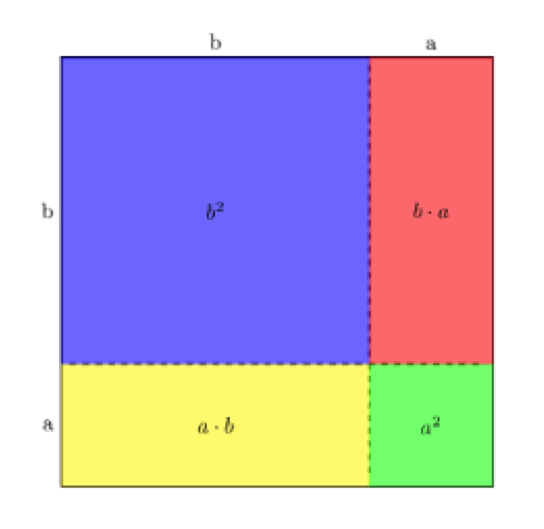
\includegraphics[width=6cm]{quadrato.eps} 
   %\label{fig:example}
$$
\centerline{ {Figura 1: $a^2+b^2+2ab = (a+b)^2$}}

}

Un altro aspetto delle verifiche è che non è richiesta una astrazione ulteriore rispetto a saper fare i conti per la verifica.
Io posso trovare una formula per un qualunque polinomio di secondo grado $ax^2+bx+c=0$, te la racconto su un esempio $2x^2+6x+10=0$,
e poi ti dico di verificare il risultato. Infine ti informo che puoi usare la stessa tecnica in generale per qualunque polinomio di secondo grado.
Tu applichi la stessa formula che avevi imparato per l'esempio anche senza capirla e poi verifichi che il risultato che trovi è giusto.
Se non ti viene la verifica, siccome la formula l'ho detta io e tu non sei un cazzo, significa che hai sbagliato tu, trovati l'errore.
Il tutto senza doverti dire cosa è l'algebra letterale con cui io faccio il conto.

\Note{Nel mondo anglosassone anche nelle discipline dure, il calcolo differenziale è ancora oggi insegnato così. Uno si fa il corso di calculus in cui impara a calcoare le derivate e gli integrali senza capire nulla. Poi si fa il corso di Analysis in cui si dimostrano i teoremi necessari a capire quello che si è imparato a fare. Per me pessima idea e un pessimo esempio di controeducazione civica. Ma è così. Questo è per me il secondo motivo per cui dovrebbe essere vietato insegnare matematica come è insegnata nella maggior parte dei casi.
}


Quindi dal 1200 ad almeno tutto il 1600 la matematica è la storia di una coppia di separati in casa, e di conseguenza la didattica della matematica un disastro.

Ora il nostro prossimo obiettivo è quello di arrivare a risolvere le equazioni di primo e secondo grado in generale.
La buona notizia è che se vi ricordate la definizione di relazione di equivalenza non avete bisogno di altro.


\EndDocument
\end


